\chapter{Load cell design comparison
\label{chap:8}}

Over the course of this program, two primary load cell designs were tested.
The first design had two electrodes seperated by a thin, 25 $\mu$m, layer of polyimide.
The second design had a single electrode coated in soldermask 
and attached to a thicker, 100 $\mu$m, layer of polyimide.
Both designs were tested in a load frame prior to rock cutting use,
and comparable XY plots are shown for both the first and second design
in \ref{fig:xycompare}. The first design is the ``Dynamic Flex Configuration'' 
and the second is the ``Air Gap Configuration''.

The first design was already very thin when it when into the rock cutting test.
The nonlinear deformation characteristics of the thin film made it difficult to determine
cutting forces, but still allowed frequency analysis for determining material type and tool wear.
The second design ultimately altered to the ``Crushed Gap Configuration'' when used for rock cutting.
This final form had even greater sensitivity and linearity, which allowed estimation of cutting forces.

Measurements for individual sensor channels and the measured 
and estimated forces are shown in \ref{fig:sense_chans}.
When attempting to estimate the rock cutting forces to determine material type and tool wear, 
the problem can be relaxed to estimating average cutting force, as the differences in 
cutting force between the conditions are great.
The cutting force bandwitdth was limited to 10 Hz for the study, as this is believed to still
provide an adequeate response time while providing good averaging.

Force on the cutting tool is determined by the tool geometry and the material.
The force is also influenced by the dynamics of the machine.
The physical sensor system also has dynamics, and depending on the model, 
these dynamics can be non-stationary.
The first design that was tested had non-linear, non-stationary dynamics.
The second design was more linear and the bias could be tracked and compensated.

The air gap design could work for applications with more gentle load profiles,
but considering that the gap will be crushed when exposed to rock cutting forces 
means that this aspect of the design is unnessacery. The first sensor design
has a high bandwidth due to its thin film. 
High bandwidth sensing is good for frequency analysis methods.
More linear and robust sensors are generally bulkier, but at the cost of sensitivity.
By starting with a thick polyimide film and allowing it to be compressed during the application,
we get a robust sensor that is stiffer and more sensitive than the original design.


\begin{figure}[ht]
\centering
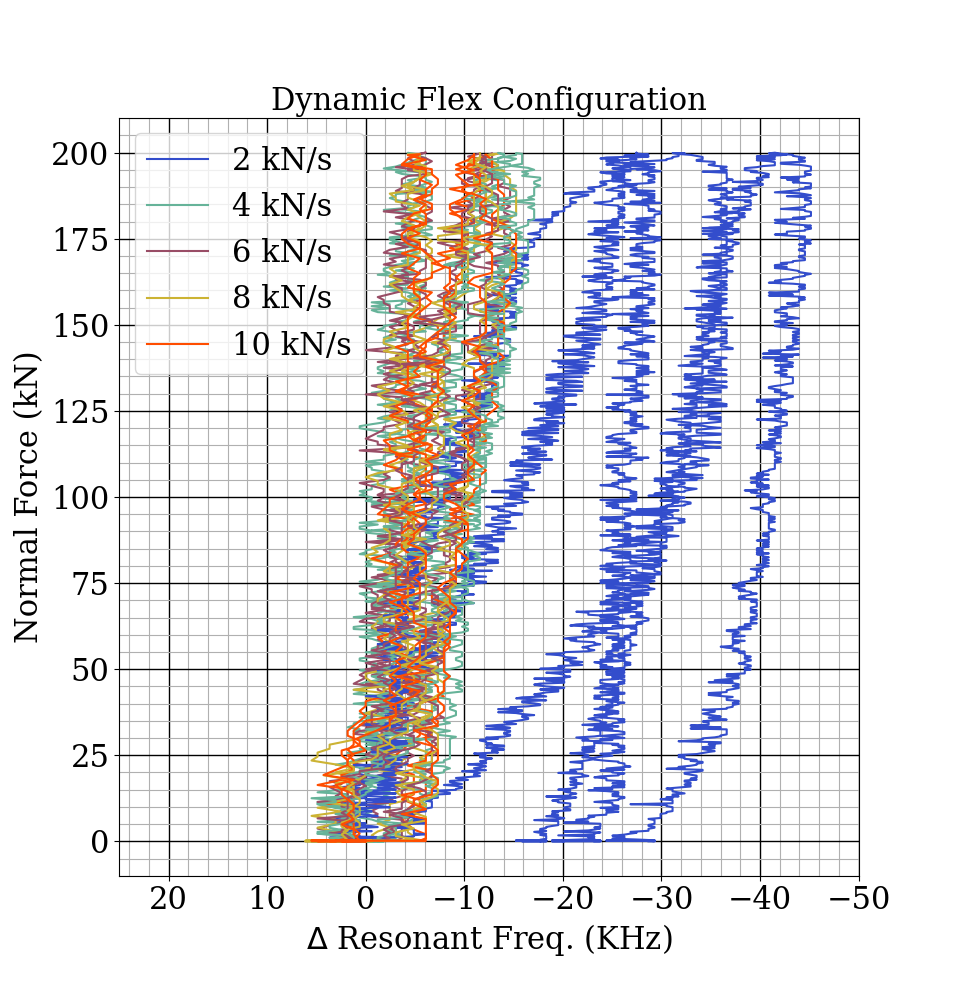
\includegraphics[width=3.0in]{ch8_flexcell.png}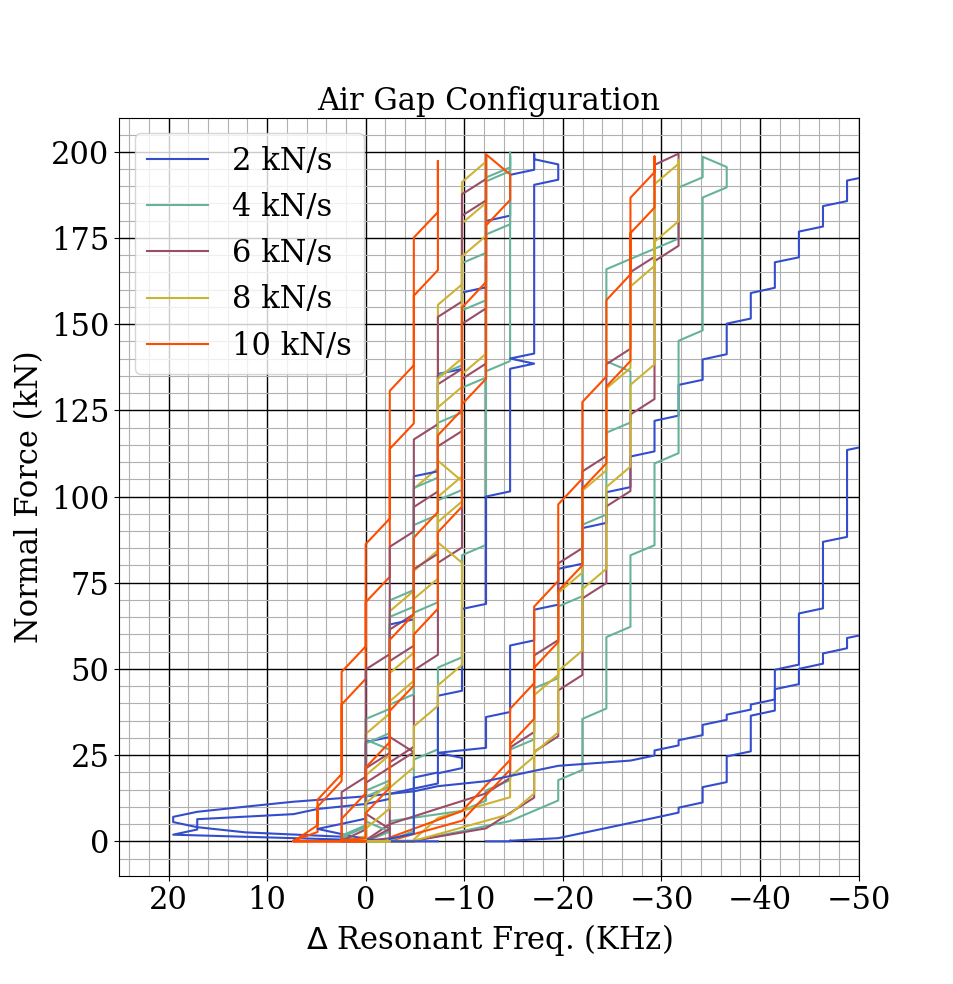
\includegraphics[width=3.0in]{ch8_airgap.png}
\caption{
Comparison of original design, left, and improved design, right.
The original design was noisy, had slightly less initial plastic deformation,
and similar sensitivity when compared to the improved ``Air Gap Configuration''.
The air gap design had much better repeatability and less hysteresis in comparison 
to the original.
The air gap design ultimately became more sensitive when used in the rock cutting tests.
}
\label{fig:xycompare}
\end{figure}



\begin{figure}[h]
\centering
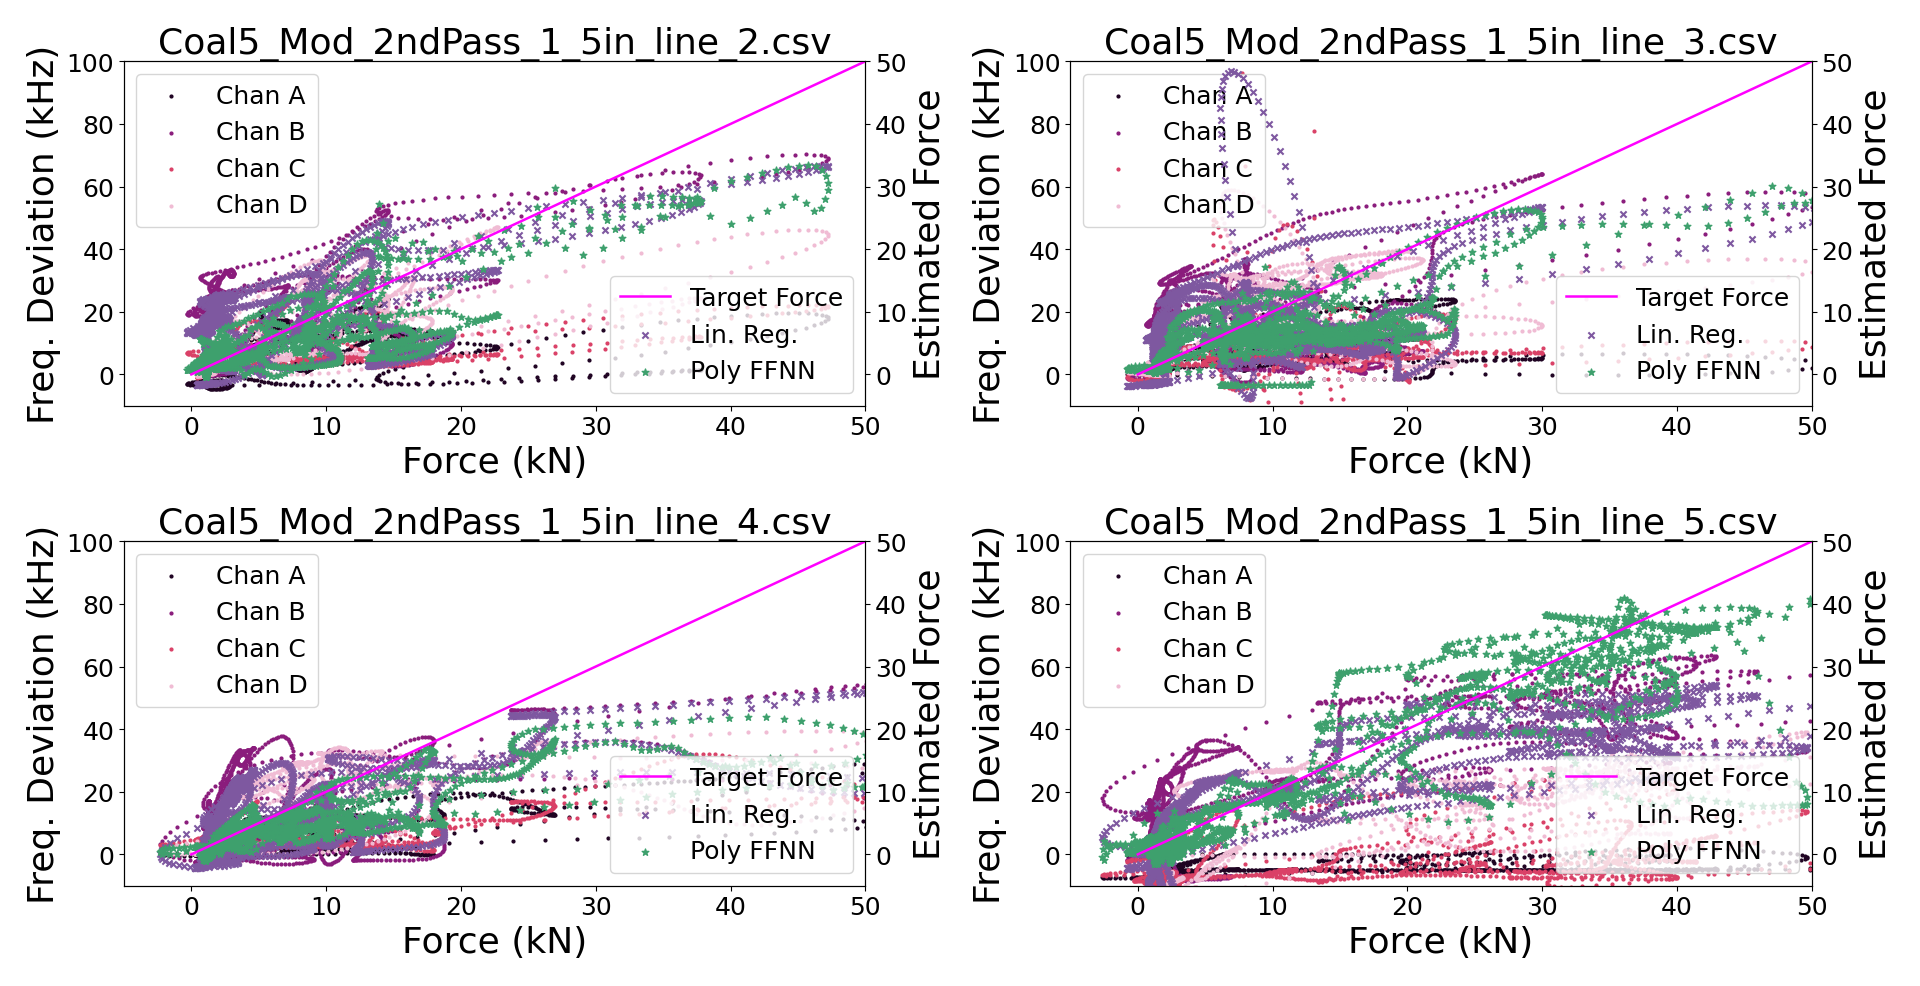
\includegraphics[width=5.5in]{ch8_sense_vals.png}
\caption{
The individual channel measurements and the resulting force predictions for a few choice cuts,
using the ``Crushed Gap Configuration'' of the second sensor design.
The change in resonant frequency from the initial value is plotted versus the target force
for each sensing channel in the sensor. The resulting force estimate provided by both the 
linear regression and the neural network using the 2nd order polynomial expansion are shown.
Ideal performance is shown along the magenta line. 
The neural network method is able to untangle some of the nonlinearities in the response.
The performance of the neural network is comparable to the strictly linear model.
The sensor is not completely linear, but can still provide useful measurements using a linear model.
}
\label{fig:sense_chans}
\end{figure}

